\documentclass{article}
\usepackage{tikz}
\usetikzlibrary{arrows.meta}

\begin{document}

\begin{figure}[h]
    \centering
    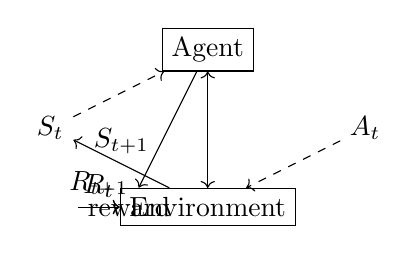
\begin{tikzpicture}[node distance=2cm, auto]
        % Define nodes
        \node (agent) [draw] {Agent};
        \node (env) [draw, below of=agent] {Environment};
        \node (state) [left of=agent, yshift=-1cm] {$S_t$};
        \node (reward) [below of=agent, xshift=-1cm] {reward};
        \node (action) [right of=agent, yshift=-1cm] {$A_t$};
        
        % Draw edges
        \draw[->] (agent) -- (env);
        \draw[->] (env) -- (agent);
        \draw[->] (agent) -- node[above] {} (reward);
        \draw[->] (reward) -- node[above] {$R_t$} (env);
        \draw[->] (reward) -- node[above] {$R_{t+1}$} (env);
        \draw[->] (env) -- node[above] {$S_{t+1}$} (state);
        \draw[->, dashed] (state) -- node[above] {} (agent);
        \draw[->, dashed] (action) -- node[above] {} (env);
    \end{tikzpicture}
    \caption{Basic agent-environment relationship in a Markov decision process. The agent chooses an action \( A_t \) and the environment returns a new state \( S_{t+1} \) and a reward \( R_{t+1} \). The dotted line represents the transition from step \( t \) to step \( t+1 \) \cite{suttonbarto}.}
\end{figure}

\end{document}